
\documentclass[a4paper,12pt]{article}
\usepackage[a4paper,top=1.3cm,bottom=2cm,left=1.5cm,right=1.5cm,marginparwidth=0.75cm]{geometry}
\usepackage{cmap}					
\usepackage[warn]{mathtext} 		
\usepackage[T2A]{fontenc}			
\usepackage[utf8]{inputenc}			 
\usepackage[english,russian]{babel}	
\usepackage{longtable}
\usepackage{float}
\restylefloat{table}
\usepackage{graphicx}
\usepackage{tabularx}
\usepackage{hyperref}
\usepackage[rgb]{xcolor}
\usepackage{amsmath,amsfonts,amssymb,amsthm,mathtools} 
\mathtoolsset{showonlyrefs=true}
\usepackage{euscript}
\usepackage{mathrsfs}
\date{\today}
\begin{document}

\begin{titlepage}
	\begin{center}
		{\large МФТИ}
	\end{center}
	\begin{center}
		{\large ФРКТ}
	\end{center}
	
	
	\vspace{4.5cm}
	{\huge
		\begin{center}
			{\bf Лабораторная работа 2.2-2.3}\\
			Изучение спектров водорода и молекулы йода.
		  
		

		\end{center}
	}
	\vspace{9cm}
	\begin{flushright}
		{\LARGE  $\newline$Добровольская Ксения$\newline$Гаврилин Илья$\newline$
			\vspace{0.2cm}
			Б01-110$\newline$}
	\end{flushright}
	\vspace{8cm}
	
\end{titlepage}

\section{Аннотация}


  В данной работе исследовались: а.) сериальные закономерности в оптическом спектре водорода, по результатам которых была рассчитана постоянная Ридберга; б.) спектр поглощения паров йода в видимой области, по результатам которого были вычислены энергия колебательного кванта молекулы йода, энергия её диссоциации в основном и возбужденном состояниях.
  
  
\section{Изучение спектра атома водорода} 
   
   
     Схема экспериментальной установки приведена на рис.1.
  
    \begin{figure}[H]
  \begin{center}
    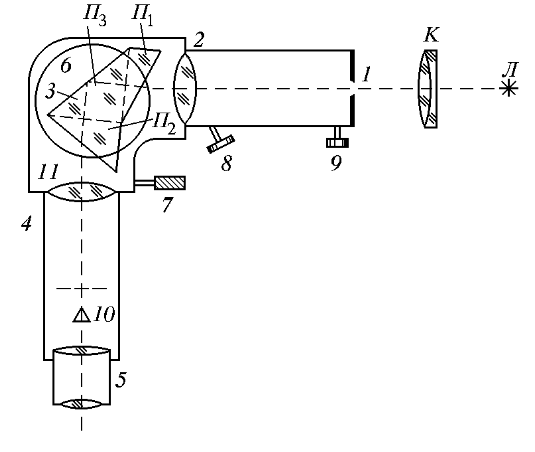
\includegraphics[width=7cm]{ex1.png}
    \caption{Схема экспериментальной установки для изучения водорода.}
    \label{fig:}
  \end{center}
\end{figure}

 
 Для измерения длин волн спектральных линий в работе используется стеклянно-призменный монохроматор-спектрометр УМ-2, преднозначенный для спектральных исследований в диапазоне от 0.38 до 1.00 мкм.
 
 В опытах по измерению длин волн бальмеровской серии источником света служит водородная трубка Н-образной формы, питаемая от источника высокого напряжения. Молекулы воды в электрическом разряде разлагаются, образуя атомарный водород. Трубка заполняется газом до давления 5-10 Торр.
 
 
 

\section{Изучение молекулярного спектра йода} 
  
  Схема экспериментальной установки приведена на рис.2.
  
    Молекулярный спектр поглощения паров йода можно наблюдать, используя
  
1.\textbf{Источник сплошного спектра} — лампу накаливания.

2.\textbf{Поглощающую среду} — кювету с исследуемым веществом.

3.\textbf{Спектральный прибор}, регристрирующий спектр поглощения - монохроматор УМ-2.

В нашей работе спектр поглощения паров йода наблюдается визуально на фоне сплошного спектра лампы накаливания 1, питаемой от блока питания 2.

Кювета 3 с кристаллами йода подогревается нихромовой спиралью, подключенной вместе с лампой накаливания к блоку питания. Линза 4 используется как конденсатор. 

В результате подогрева кристаллы йода частично возгоняются, образуя пары с легкой фиолетовой окраской. Спектрометр позволяет визуально наблюдать линии поглощения молекул йода на фоне сплошного спектра излучения лампы накаливания видимой области.

  
      \begin{figure}[H]
  \begin{center}
    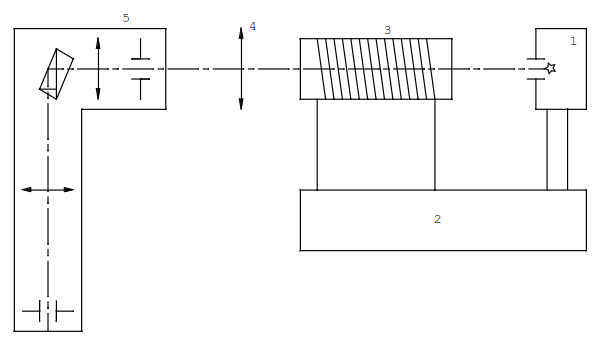
\includegraphics[width=8cm]{ex2.png}
    \caption{Схема экспериментальной установки для изучения йода.}
    \label{fig:}
  \end{center}
\end{figure}



\section{Ход работы} 
  
 
 \begin{enumerate}
\item Калибруем барабан спектрометра по спектру неона:

  \begin{table}[H]
\begin{center}
\begin{tabular}{|c|c|c|c|c|c|c|c|c|c|c|c|c|}
\hline $N $&1 &2&3&4&5&6&7&8&9&10&11&12\\
\hline $\varphi , ^{o}$&2536&2566&2500&2490&2462&2440&2430&2394&2386&2366&2354&2338\\
\hline $\lambda , A$&7032&6929&6717&6678&6599&6533&6506&6402&6383&6334&6305&6266\\
\hline 
\end{tabular}
\end{center}
\end{table}

       \begin{figure}[H]
  \begin{center}
    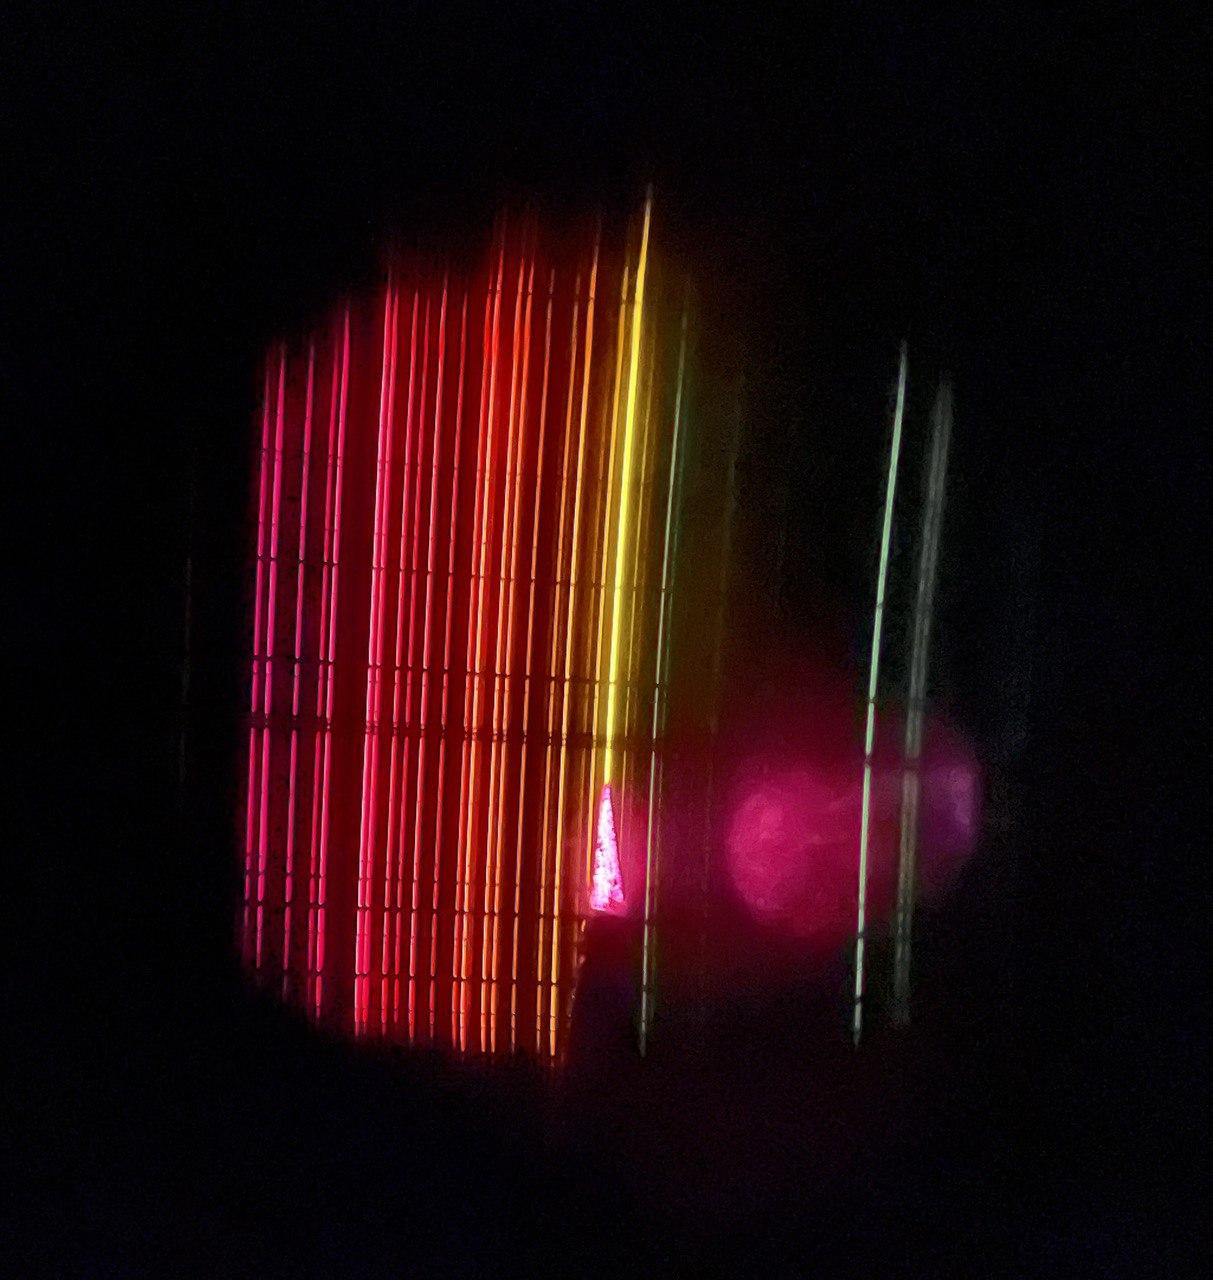
\includegraphics[width=12cm]{ex3.jpg}
    \caption{Спектр неона.}
    \label{fig:}
  \end{center}
\end{figure}

  \begin{table}[H]
\begin{center}
\begin{tabular}{|c|c|c|c|c|c|c|c|c|c|c|c|c|}
\hline $N $&13 &14&15&16&17&18&19&20&21&22&23&24\\
\hline $\varphi , ^{o}$&2320&2298&2290&2270&2262&2240&2212&2200&2170&2158&1896&1856\\
\hline $\lambda, A
$&6217&6164&6143&6096&6074&6030&5976&5945&5882&5853&5401&5331\\
\hline 
\end{tabular}
\end{center}
\end{table}

\item Строим градуировочную кривую:

       \begin{figure}[H]
  \begin{center}
    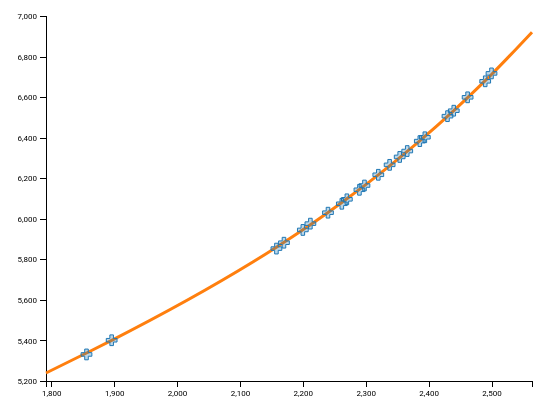
\includegraphics[width=13cm]{gra1.png}
    \caption{Градуировочная кривая по спектру неона. $\lambda, A(\varphi, ^{o})$}
    \label{fig:}
  \end{center}
\end{figure}




\item Калибруем барабан спектрометра по спектру ртути:

  \begin{table}[H]
\begin{center}
\begin{tabular}{|c|c|c|c|c|c|c|c|c|}
\hline $N $&K1&K2&1&2&3&4&5&6\\
\hline $\varphi, ^{o}$&2572&2328&2136&2134&1936&1526&858&320\\
\hline $\lambda, нм$&691&623&579&577&546&492&436&405\\
\hline 
\end{tabular}
\end{center}
\end{table}


      \begin{figure}[H]
  \begin{center}
    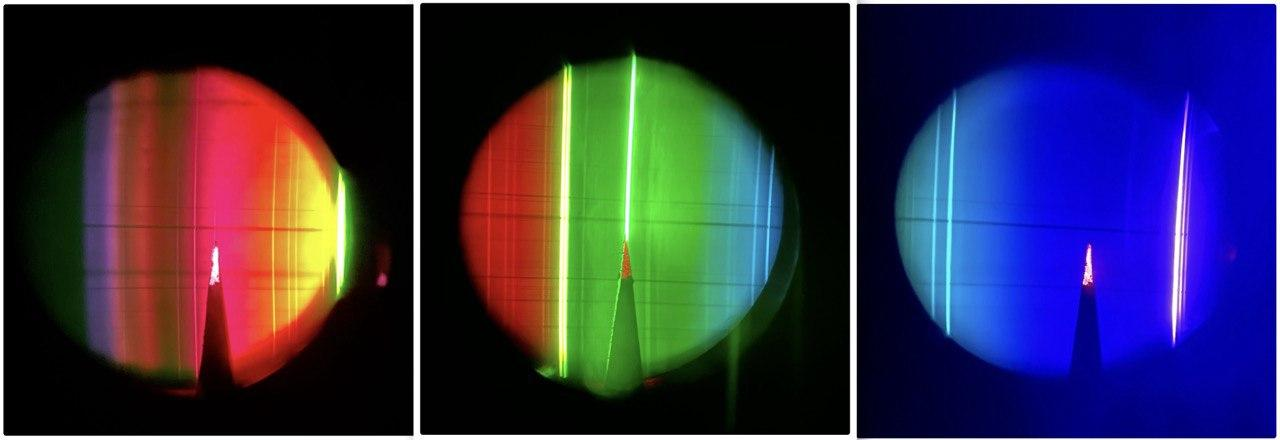
\includegraphics[width=15cm]{ex4.jpg}
    \caption{Спектр ртути.}
    \label{fig:}
  \end{center}
\end{figure}

\item Строим градуировочную кривую:

       \begin{figure}[H]
  \begin{center}
    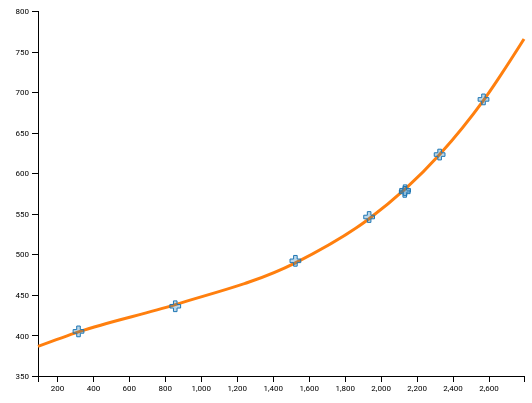
\includegraphics[width=15cm]{gra2.png}
    \caption{Градуировочная кривая по спектру ртути. $\lambda, nm(\varphi, ^{o})$}
    \label{fig:}
  \end{center}
\end{figure}

\item Определяем координаты линий бальмеровской серии атомарного водорода (n = 2, Z = 1):

  \begin{table}[H]
\begin{center}
\begin{tabular}{|c|c|c|c|c|}
\hline Название&$H_{\alpha}$&$H_{\alpha}$&$H_{\alpha}$&$H_{\alpha}$\\
\hline Цвет&красный&голубой&фиолетовый&не видна\\
\hline $\varphi , ^{o}$&2448&1458&820&-\\
\hline $R, (cm)^{-1}$&110770&113400&108180&-\\
\hline $\lambda , A$&6500&4700&4400&-\\
\hline $m$&3&4&5&6\\
\hline $k$&7.2&5.33&4.76&4.5\\
\hline 
\end{tabular}
\end{center}
\end{table}

\item Из градуировочных кривых определяем длины волн бальмеровской серии атомарного водорода. Отношения длин волн cоответствуют формуле сериальной закономерности.


\item По результатам предыдущих измерений рассчитываем постоянную Ридберга для каждой из наблюдаемых линий водорода.

\[R = \frac{1}{\lambda_{mn} Z^2 (\frac{1}{n^2} - \frac{1}{m^2})} = \frac{k_{mn}}{\lambda_{mn} Z^2}\]

Среднее значение R = $110800 \pm 1500 (cm)^{-1}$. Данный результат соответствует табличному значению R = 109 678 $(cm)^{-1}$ в рамках погрешности.


\item Определяем деления барабана монохроматора, соответсвующие первой $S_1$ и шестой $S_6$ линиям молекулярного спектра йода. Кордината приблизительного конца отчетливой видимости спектральных линий $S_gr$. h = 4.1 $*10^{-15}$эВ с


  \begin{table}[H]
\begin{center}
\begin{tabular}{|c|c|c|c|c|}
\hline &$\varphi, ^{o}$&$\lambda ,A$&$\nu = \frac{c}{\lambda} ,10^{14} Gts $&$h\nu, eB$\\
\hline $S_1$&2326&6170&4.86&1.99\\
\hline $S_6$&2224&5980&5.02&2.06\\
\hline $S_{gr}$&1702&5100&5.88&2.41\\

\hline 
\end{tabular}
\end{center}
\end{table}


\item По результатам предыдущих измерений вычисляем энергию колебательного кванта молекулы йода и энергию её диссоциации в основном и возбужденном состояниях:

\[h\nu_2 = \frac{h\nu_06 - h\nu_01}{5} = 0.013 eB\]

Используем, что энергия колебательного кванта основного состояния = $h\nu_1$ = 0.027 эВ, энергия возбуждения атома $E_a$ = 0.94 эВ, $h\nu_{gr}$ = 2.44 эВ, энергия диссоциации молекулы йода $E_d$ = 1.5 эВ.

Энергия электронного перехода 

\[h\nu_01 = h\nu_{el} + h\nu_2 (n_2 + \frac{1}{2}) - \frac{1}{2}h\nu_1 = h\nu_{el} + \frac{1}{2}(h\nu_2 - h\nu_1)\]

\[h\nu_{el} = h\nu_01 + \frac{1}{2}(h\nu_1 - h\nu_2) = 1.99 + 0.007 = 2 eB\]

Энергия диссоциации молекулы в основном состоянии

\[D_1 = h\nu_{gr} - E_a = 2.44 - 0.94 = 1.5 eB\]

Табличное значение 1.5425 эВ.

в возбужденном

\[D_2 = h\nu_{gr} - h\nu_{el} = 2.44 - 2 = 0.44 eB\]

Табличное значение 0.69 эВ. 


\end{enumerate}



\section{Выводы}

В данной работе мы 
$\newline$
1.) Исследовали сериальные закономерности в оптическом спектре водорода, с помощью проградуированного монохроматора рассчитали значения длин волн бальмеровской серии атомарного водорода и получили соответствие формуле сериальной закономерности. По результатам этих рассчетов вычислили постоянную Ридберга, ее значение составило R = $110800 \pm 1500 (cm)^{-1}$, что с учетом погрешности соответсвует табличному значению.


2.) Спектр поглощения паров йода в видимой области. Были вычислены энергия колебательного кванта молекулы йода, энергия её диссоциации в основном и возбужденном состояниях. Значения данных по порядку величин сходятся с табличными.


\end{document}
	
